
\section{Demonstration}

\begin{figure*}
\centering
 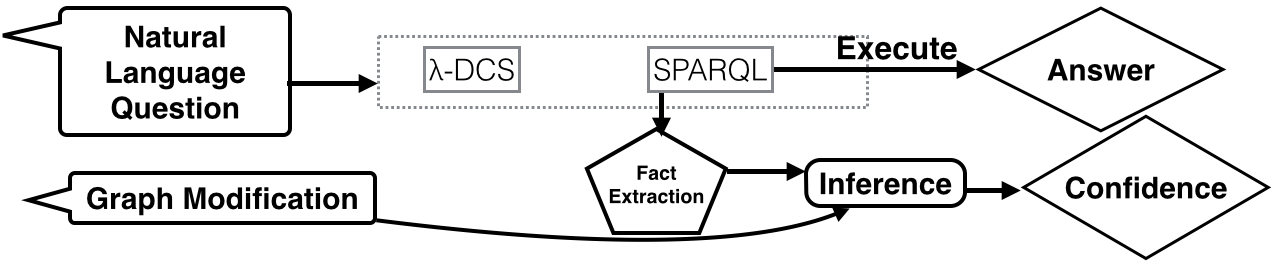
\includegraphics[width=0.9\linewidth]{images/probqa-pipeline.png}
 \caption{Probabilistic knowledge base assisted question answering demonstration pipeline.}
\label{fig:probqa-pipeline}
\end{figure*}

%The framework is developed using AngularJS\@ to completely compatible with desktop and mobile devices.
The interface allows users to make queries using three different modalities.
Users will be able to enter natural language questions, search through the set of existing facts, and use a graph to explore connections between graphs.
New probabilistic facts and rules can also be added to the system through the interface.
Users can also remove or alter the existing facts and rerun queries.
The status of queries and the underlying processes are displayed on the main interface.


We can visualize the ranking of candidates with each candidates truthfulness value.

Describe D3 visualization of graph and rule display
Describe user interaction with graph
Describe user selecting facts
Describe users removing facts


Features
  Add the auto complete for previous questions.

Describe how users will be able to alter parameters.
Add figure of the pipeline process and the user interface.


Describe the PostgreSQL database and the other services running on servers.
Describe the tables 
Describe the functions that are called
Describe the parallelism

The system is loaded with docker, a system container, so any modifications by demo can be quickly rolled back to the initial state.





